\renewcommand\appendixpagename{Appendix}
\appendix
%\appendixpagename

%\addappheadtotoc


\titleformat{\chapter}{\normalfont\LARGE\scshape}{Appendix \thechapter: }{.1em}{\vspace{1ex}}[\titlerule]
% appendixes go here
\begin{appendices}
\chapter{Glossary}
  \begin{itemize}
    \item{Unsupervised Learning: the use of algorithms on unlabeled data to obtain clusters, or groupings, that partition the data.}
  
    \item{Supervised Learning: the use of algorithms on labeled data to classify (or regress) data into categories (or estimate values).}
  
    \item{Bigram/N-Gram: a pair of two words which appear adjacent to one another in text. Generalized to $n$ words appearing adjacent to one another, in sequence.}

  \end{itemize}
\chapter{Session Info - R}

\begin{lstlisting}
> sessionInfo()
R version 4.0.3 (2020-10-10)
Platform: x86_64-apple-darwin19.6.0 (64-bit)
Running under: macOS Big Sur 10.16

Matrix products: default
LAPACK: /usr/local/Cellar/r/4.0.3/lib/R/lib/libRlapack.dylib

locale:
[1] en_US.UTF-8/en_US.UTF-8/en_US.UTF-8/C/en_US.UTF-8/en_US.UTF-8

attached base packages:
[1] stats     graphics  grDevices datasets  utils     methods   base     

other attached packages:
 [1] slam_0.1-47              topicmodels_0.2-11       ggraph_2.0.4             igraph_1.2.6             widyr_0.1.4             
 [6] stringdist_0.9.8         ggrepel_0.8.2            smacof_2.1-3             e1071_1.7-9              colorspace_2.0-2        
[11] plotrix_3.8-2            proxy_0.4-26             broom_0.7.10             textmineR_3.0.5          Matrix_1.3-4            
[16] SparseFactorAnalysis_1.0 proto_1.0.0              directlabels_2021.1.13   plotly_4.10.0            factoextra_1.0.7        
[21] FactoMineR_2.3           tm_0.7-8                 NLP_0.2-1                tidytext_0.3.2           tidyr_1.1.4             
[26] DT_0.16                  stringr_1.4.0            purrr_0.3.4              readr_1.4.0              dplyr_1.0.7             
[31] ggplot2_3.3.5            here_1.0.1              

loaded via a namespace (and not attached):
  [1] backports_1.4.0      Hmisc_4.6-0          VGAM_1.1-5           plyr_1.8.6           lazyeval_0.2.2       splines_4.0.3       
  [7] crosstalk_1.2.0      SnowballC_0.7.0      candisc_0.8-6        digest_0.6.28        foreach_1.5.1        htmltools_0.5.2     
 [13] viridis_0.6.2        gdata_2.18.0         fansi_0.5.0          magrittr_2.0.1       checkmate_2.0.0      cluster_2.1.2       
 [19] doParallel_1.0.16    graphlayouts_0.7.1   wordcloud_2.6        jpeg_0.1-9           xfun_0.28            crayon_1.4.2        
 [25] jsonlite_1.7.2       lme4_1.1-27.1        survival_3.2-13      iterators_1.0.13     glue_1.5.0           polyclip_1.10-0     
 [31] stopwords_2.3        gtable_0.3.0         nnls_1.4             car_3.0-12           weights_1.0.4        abind_1.4-5         
 [37] scales_1.1.1         rstatix_0.6.0        Rcpp_1.0.7           viridisLite_0.4.0    htmlTable_2.3.0      flashClust_1.01-2   
 [43] foreign_0.8-81       Formula_1.2-4        stats4_4.0.3         heplots_1.3-9        truncnorm_1.0-8      htmlwidgets_1.5.4   
 [49] httr_1.4.2           RColorBrewer_1.1-2   modeltools_0.2-23    ellipsis_0.3.2       mice_3.13.0          pkgconfig_2.0.3     
 [55] farver_2.1.0         nnet_7.3-16          utf8_1.2.2           tidyselect_1.1.1     labeling_0.4.2       rlang_0.4.12        
 [61] reshape2_1.4.4       polynom_1.4-0        munsell_0.5.0        tools_4.0.3          cli_3.1.0            generics_0.1.1      
 [67] evaluate_0.14        fastmap_1.1.0        yaml_2.2.1           knitr_1.36           tidygraph_1.2.0      nlme_3.1-153        
 [73] leaps_3.1            xml2_1.3.2           tokenizers_0.2.1     compiler_4.0.3       rstudioapi_0.13      png_0.1-7           
 [79] ggsignif_0.6.0       tweenr_1.0.1         tibble_3.1.6         stringi_1.7.5        lattice_0.20-45      nloptr_1.2.2.3      
 [85] vctrs_0.3.8          pillar_1.6.4         lifecycle_1.0.1      data.table_1.14.2    R6_2.5.1             latticeExtra_0.6-29 
 [91] renv_0.14.0          RcppProgress_0.4.2   gridExtra_2.3        janeaustenr_0.1.5    codetools_0.2-18     boot_1.3-28         
 [97] MASS_7.3-54          gtools_3.9.2         rprojroot_2.0.2      withr_2.4.2          parallel_4.0.3       hms_0.5.3           
[103] quadprog_1.5-8       grid_4.0.3           rpart_4.1-15         class_7.3-19         minqa_1.2.4          rmarkdown_2.11      
[109] carData_3.0-4        ggpubr_0.4.0         ggforce_0.3.2        scatterplot3d_0.3-41 base64enc_0.1-3      ellipse_0.4.2       
\end{lstlisting}

\chapter{Example Code} 

\begin{lstlisting}
\# Calculating the cosine similarity/distance matrix
cos_mat <- stringdistmatrix(course_full_desc$text, course_full_desc$text, 
useNames = FALSE, method = "cosine") %>% 
  as.matrix()

colnames(cos_mat) <- course_full_desc$Course_ID
rownames(cos_mat) <- course_full_desc$Course_ID

cos_course <- reshape2::melt(cos_mat)[reshape2::melt(upper.tri(cos_mat))$value,]

colnames(cos_course) <- c("Term1", "Term2", "distance")


# Plotting 
cos_course %>% 
  filter(distance < 0.02) %>% 
  graph_from_data_frame() %>%
  ggraph(layout = "fr") +
  geom_edge_link(aes(edge_alpha = distance), show.legend = FALSE) +
  geom_node_point(color = "lightblue", size = ptsize) +
  geom_node_text(aes(label = name), repel = TRUE) +
  theme_void() + 
  labs(title = "1 - Cosine Similarity Plot: Full Desc.")

ggsave("img/cos.png", dpi = 300)


# Calculating the Jaccard similarity/distance matrix
jac_mat <- stringdistmatrix(course_full_desc$text, course_full_desc$text, useNames = FALSE, method = "jaccard") %>% 
  as.matrix()

colnames(jac_mat) <- course_full_desc$Course_ID
rownames(jac_mat) <- course_full_desc$Course_ID

jac_course <- reshape2::melt(jac_mat)[reshape2::melt(upper.tri(jac_mat))$value,]

colnames(jac_course) <- c("Term1", "Term2", "distance")

# Plotting
jac_course %>% 
  filter(distance < 0.04) %>% 
  graph_from_data_frame() %>%
  ggraph(layout = "fr") +
  geom_edge_link(aes(edge_alpha = distance), show.legend = FALSE) +
  geom_node_point(color = "lightblue", size = ptsize) +
  geom_node_text(aes(label = name), repel = TRUE) +
  theme_void() + 
  labs(title = "1 - Jaccard Similarity Plot: Full Desc.")

ggsave("img/jac.png", dpi = 300)

# MDS
mds_cos_mat <- cos_mat %>% 
  mds(type = "ordinal")

ggplot() +
  geom_point(data = as_tibble(mds_cos_mat$conf), aes(x = D1, y = D2, 
  colour = D2 > 0.5)) +
  scale_colour_manual(values = setNames(c('#532d8e','grey'),c(T, F))) +
  scale_alpha_manual(values = c(1, 0.01)) +
  geom_text(as_tibble(mds_cos_mat$conf), mapping = aes(
    x = -D1, y = -D2, color = D2 < -0.5, label = paste(rownames(cos_mat))), alpha = .7) +
  geom_text_repel() +
  theme_minimal() +
  labs(title = "MDS with 1 - Cosine Similarity") +
  theme(legend.position = "")

ggsave("img/cos_mds.png", dpi = 300) 

# Fitting an LDA topic model
# k = 5 for the number of concentrations
bigram_lda <- LDA(bigram_dtm, k = 5, method = "Gibbs", control=list(iter = 500, verbose = 25, alpha = 0.2))
 

\end{lstlisting}

\chapter{Mechanical Engineering and Environmental Engineering Plan of Study}

Mechanical Engineering and Environmental Engineering has less programming courses and emphasizes more math related courses. Again, we fit a topic model 
to find the number of concentrations (k = 5). Figure \ref{fig:lda_me} shows the model's performance on this plan of study. Here is a list of the concentrations:

\begin{itemize}
  \item Advanced Topics
  \item Aerospace Engineering
  \item Materials and Advanced Manufacturing
  \item Mechanical and Thermal Systems
  \item Operations Research 
\end{itemize}

\begin{figure}[H]
  \centering
  
  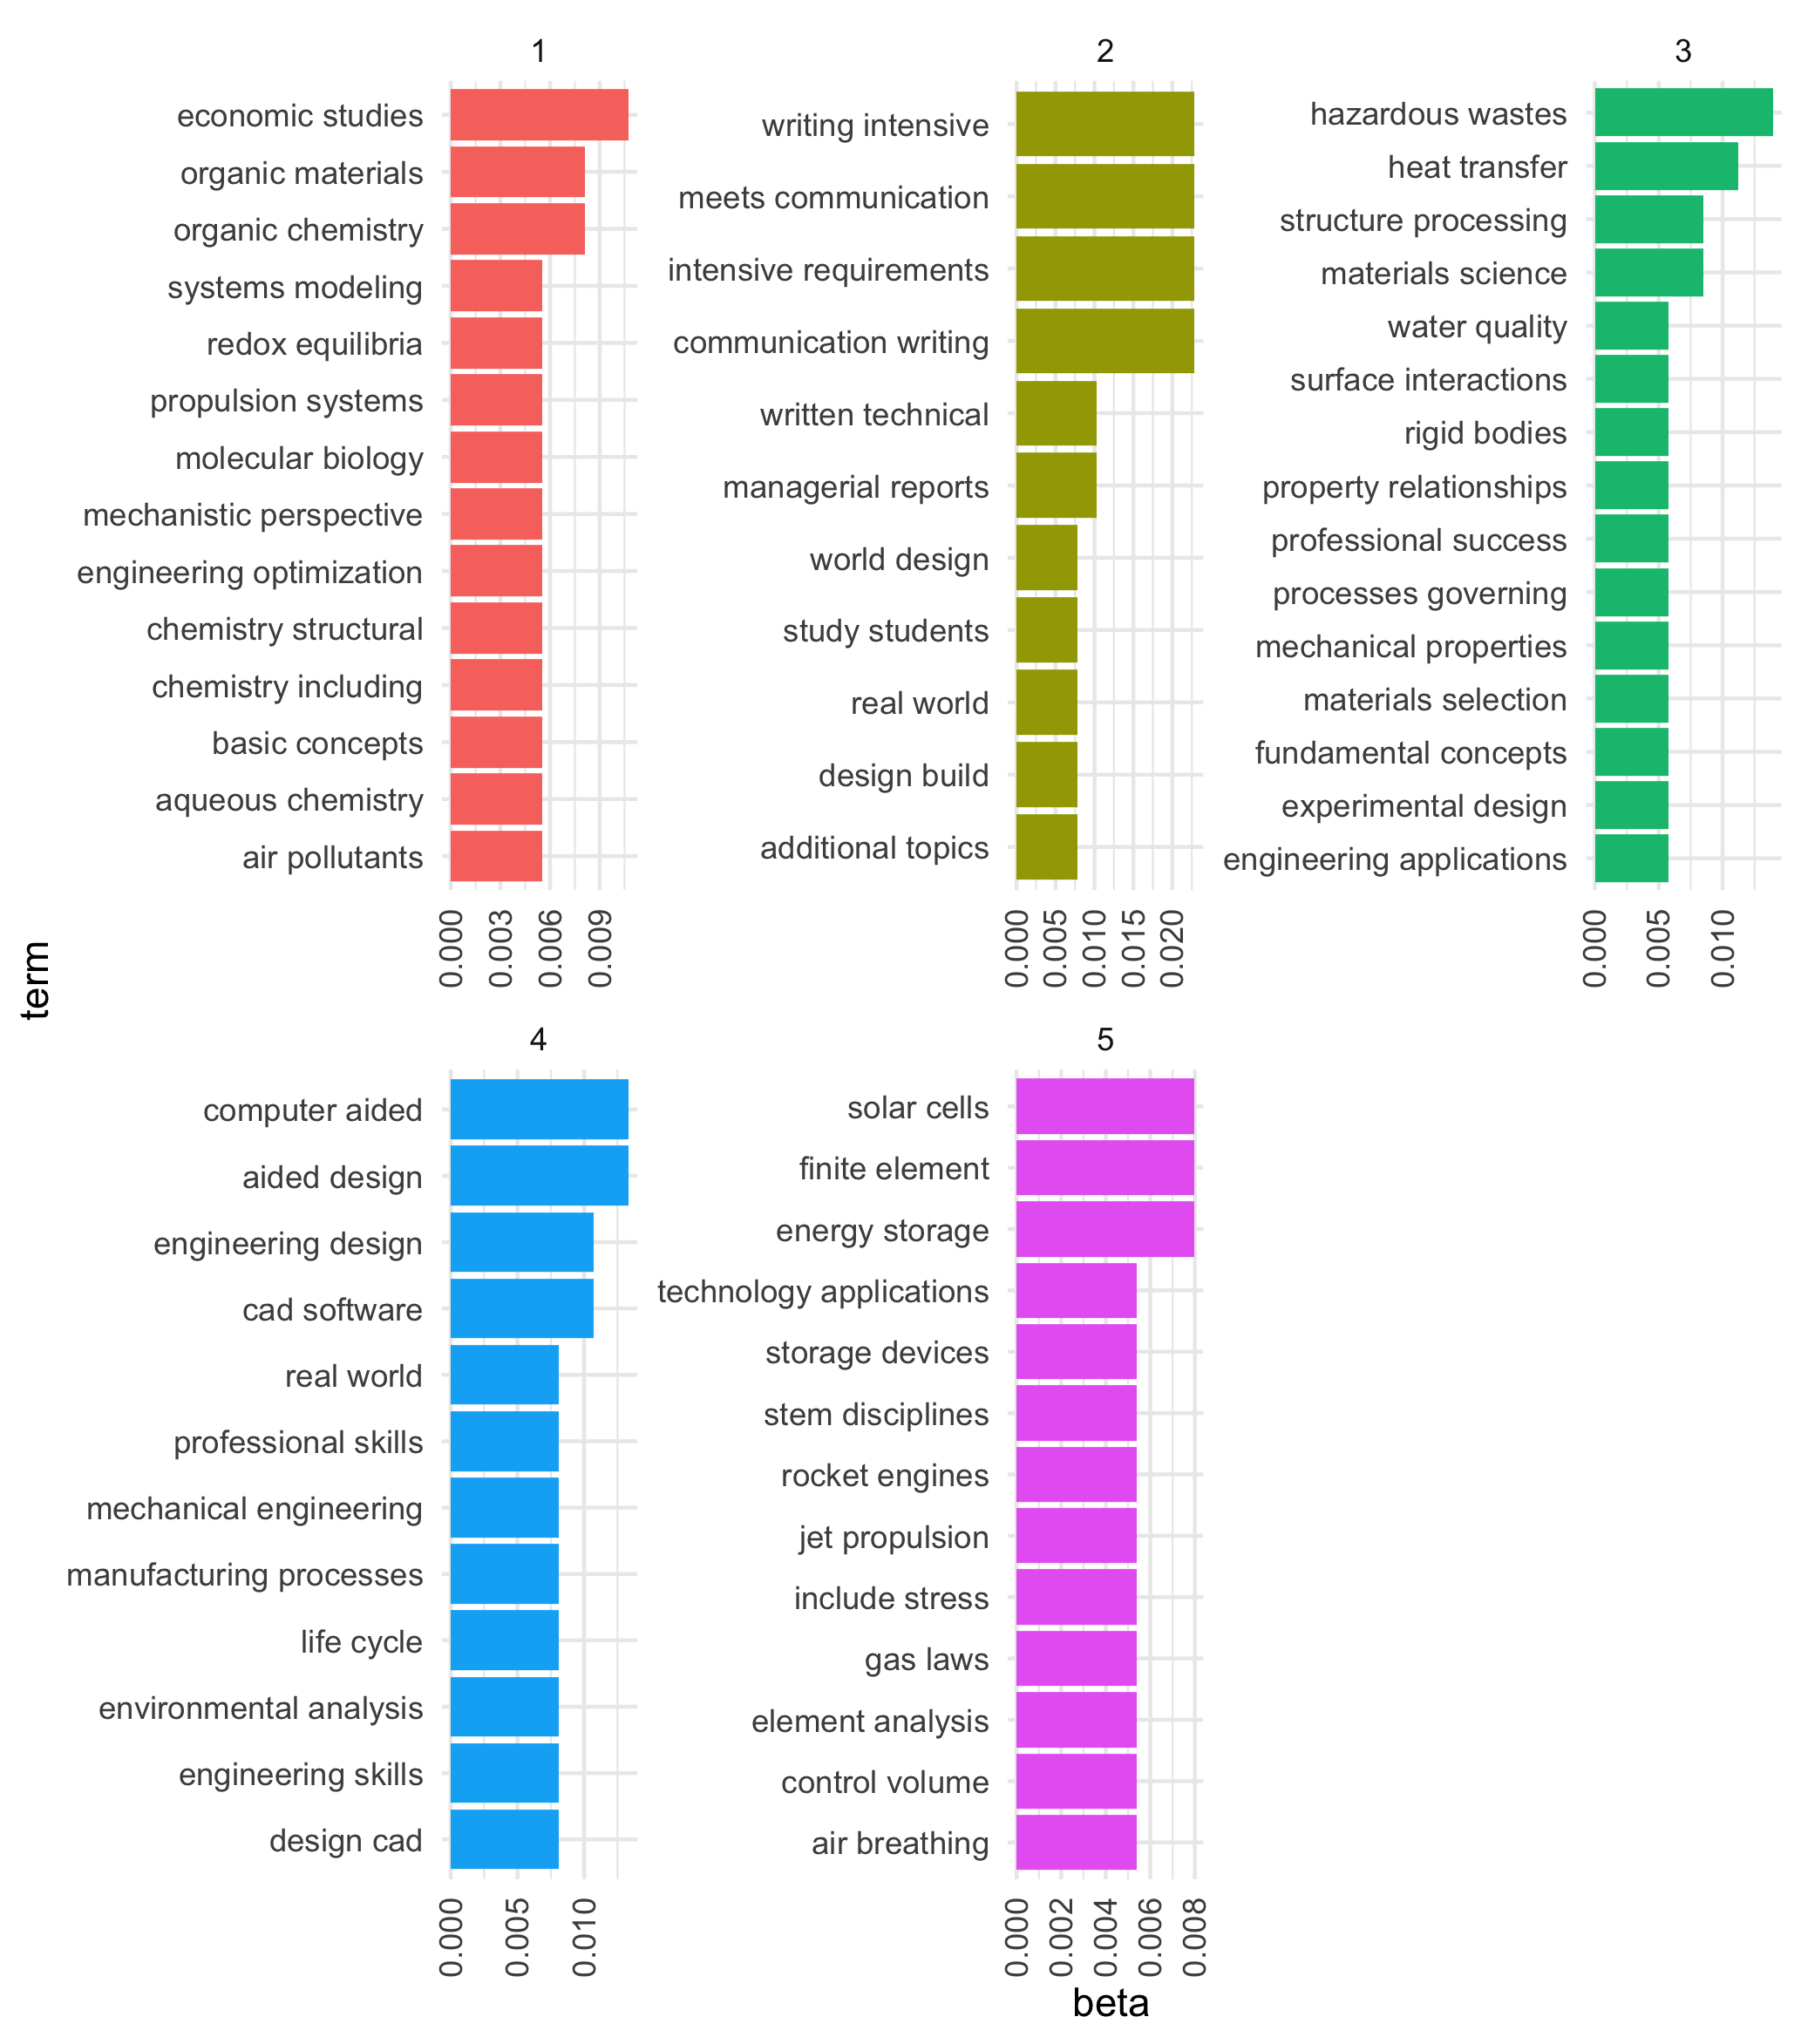
\includegraphics[width = .8\textwidth, height = .7\textheight]{Content/images/lda_me.png}
  \caption{LDA topic model splitting course topics into concentrations for the Mechanical Engineering Plan of Study}
  \label{fig:lda_me}
\end{figure}

\end{appendices}